% Compile: pdflatex poc_report && bibtex poc_report && pdflatex poc_report && pdflatex poc_report
\documentclass[12pt]{article}
\usepackage{graphicx}
% \usepackage{geometry}
% \geometry{left=2cm, right=2cm, top=1cm, bottom=1cm}
\usepackage[utf8]{inputenc}
\usepackage{float}
\usepackage{placeins}
\usepackage[colorlinks=true, allcolors=blue]{hyperref}
\usepackage{fancyhdr}
\setlength{\headheight}{14.5pt}
\usepackage{tikz}
\usetikzlibrary{positioning,arrows.meta,shapes.geometric,fit,backgrounds,calc}
% \usepackage[none]{hyphenat}
\pagestyle{fancy}
% \usepackage{ragged2e}
\usepackage[english]{babel}

\fancyhf{}
\fancyhead[L]{\textbf{VoiceFL-MAML — Federated Meta-Learning for Speech Recognition}}
\fancyfoot[C]{\hspace{4cm}\thepage}

\usepackage{graphicx}
\usepackage{amsmath,booktabs,array,caption,xcolor,colortbl,multirow,siunitx}

\definecolor{lightgray}{gray}{0.9}
\newcolumntype{C}{>{\centering\arraybackslash}p{0.8cm}}

\usepackage{amsmath}
\newtheorem{example}{Example}
\usepackage{hyperref}
\graphicspath{{Figures/}}
\addtolength{\textwidth}{1in}
\addtolength{\textheight}{1in}
\addtolength{\evensidemargin}{0.5in}
\addtolength{\oddsidemargin}{-0.5in}
\addtolength{\topmargin}{-0.5in}

\title{VoiceFL-MAML: Federated Meta-Learning for\\
       Personalised Accented Speech Recognition}
\author{Hany El Atlassi - Marouane El-Hamdaoui - Rabyâ Raghib \\ \\
Supervisor : Badr Hirchoua \\}
\date{April 27, 2026}
\usepackage{mathpazo}
\renewcommand\familydefault{\rmdefault}

\usepackage{amsthm}

\theoremstyle{plain}
\newtheorem{lemma}{Fact}[section]
\newtheorem{conjecture}{Conjecture}[section]
\newtheorem{lema}{Lema}[section]

\newcommand{\jp}[1]{\textcolor{teal}{#1}}
\newcommand{\pe}[1]{{\color{red}{#1}}}
\sloppy

% Extra colours used in tables / boxes
\definecolor{NavyBlue}{HTML}{1B3A6B}
\definecolor{PastelBlue}{HTML}{D6E8F5}
\definecolor{PastelGreen}{HTML}{D5F0DC}
\definecolor{PastelRed}{HTML}{FAD7D7}
\definecolor{PastelYellow}{HTML}{FDF3D0}
\definecolor{ForestGreen}{HTML}{2D6A2D}
\definecolor{BrickRed}{HTML}{B03030}

\begin{document}
\maketitle
\thispagestyle{empty}

\begin{abstract}
We present \textbf{VoiceFL-MAML}, a two-phase federated meta-learning system for personalised automatic speech recognition of accented English. Phase~1 establishes a proof-of-concept using FOMAML-ANIL on LibriSpeech. Phase~2, \emph{FedLoRA-MAML}, deploys true second-order MAML with LoRA adapters on the L2-ARCTIC corpus, training over 12 federated nodes spanning six non-native English accent groups.
After 50 rounds the federated meta-initialisation $\theta^*$ matches or outperforms \texttt{wav2vec2-base-100h} on three of six accent groups, with a \SI{3.1}{pp} statistically significant improvement for Vietnamese (THV). Communication cost is reduced \textbf{295$\times$} relative to full Per-FedAvg by transmitting only 320K LoRA parameters per round instead of 94.5M.
Projections from the convergence curve indicate that with 200 total rounds the system may approach the performance of the much larger \texttt{wav2vec2-base-960h} baseline
on several accent groups.
\end{abstract}


\tableofcontents
\clearpage

% \listoffigures
% \newpage
% \listoftables
% \newpage

% ============================================================
\section*{Introduction}
\addcontentsline{toc}{section}{Introduction}
% ============================================================

Automatic speech recognition (ASR) systems trained on large, homogeneous corpora
generalise poorly to speakers with non-native accents.
The performance gap between native and accented English is especially severe for
speakers with L1 backgrounds that share few phonological features with American
English, Vietnamese and Arabic speakers frequently experience word-error rates
(WER) two to three times higher than native-speaker baselines.

Collecting labelled accented speech at scale and
fine-tuning conflicts with privacy requirements: voice recordings are personal
biometric data.
A speaker should not need to upload their voice to an external server in order to
receive a model calibrated to their accent.

\textbf{Federated learning} distributes training across nodes, each of which holds
private data that never leaves the device.
\textbf{Meta-learning} (MAML~\cite{finn2017maml}) goes further: instead of
training a single shared model, it trains an initialisation $\theta^*$ from which
any new speaker can adapt rapidly with just a few gradient steps.

This project implements and evaluates a system that combines both ideas:
\textbf{FedLoRA-MAML}: a federated, second-order MAML system using
Low-Rank Adaptation (LoRA~\cite{hu2022lora}) to reduce the parameter space
that must be communicated, making the system practical on commodity hardware.

\paragraph{Proof statement.} 
A federated meta-initialisation $\theta^*$ enables a \emph{new, unseen} speaker to
adapt a speech recognition model to their accent faster (lower WER with fewer
adaptation steps) than a standard pretrained baseline, while voice data never
leaves its local node.

\paragraph{Report structure.}
Section~\ref{sec:background} reviews the relevant techniques.
Section~\ref{sec:architecture} describes the system architecture.
Sections~\ref{sec:data}--\ref{sec:security} cover the data pipeline,
infrastructure, protocol, and privacy design.
Section~\ref{sec:training} documents the training journey including three
resolved failure modes.
Sections~\ref{sec:eval}--\ref{sec:projection} present results and projections.
Section~\ref{sec:conclusion} concludes.

% ============================================================
\section{Background}
\label{sec:background}
% ============================================================

\subsection{Automatic Speech Recognition and Wav2Vec2}

\texttt{wav2vec~2.0}~\cite{baevski2020wav2vec2} is a transformer-based
self-supervised model pre-trained on 960 hours of LibriSpeech audio.
It encodes raw waveforms through a CNN feature extractor followed by a 12-layer
transformer (\textasciitilde94.5M parameters) and a linear classification head
(\texttt{lm\_head}, \textasciitilde25K parameters) that maps encoder outputs to
character logits.

\paragraph{Connectionist Temporal Classification.}
Decoding is performed with CTC~\cite{graves2006ctc}, which marginalises over all
monotonic alignments between input frames and output labels:
\begin{equation}
  \mathcal{L}_{\mathrm{CTC}}(\theta) =
    -\log \sum_{\pi \in \mathcal{B}^{-1}(y)} \prod_{t=1}^{T} p(\pi_t \mid x;\theta),
\end{equation}
where $\mathcal{B}$ collapses repeated tokens and blank symbols.

We use two fine-tuned checkpoints as baselines:
\texttt{wav2vec2-base-100h} (fine-tuned on 100 hours of labelled LibriSpeech)
and \texttt{wav2vec2-base-960h} (the full 960-hour corpus).
Our federated model is initialised from the 100h checkpoint, chosen because it
provides a trained \texttt{lm\_head} while still leaving substantial room for
meta-learning improvement.

\subsection{Meta-Learning and MAML}

Model-Agnostic Meta-Learning (MAML)~\cite{finn2017maml} aims to find a parameter
initialisation $\theta$ such that a small number of gradient steps on a new
task produce strong performance.
Given a distribution of tasks $p(\mathcal{T})$, the outer-loop objective is:
\begin{equation}
  \min_\theta \sum_{\mathcal{T}_i \sim p(\mathcal{T})}
    \mathcal{L}^{\mathcal{T}_i}\!\left(
      \theta - \alpha \nabla_\theta \mathcal{L}^{\mathcal{T}_i}(\theta)
    \right).
\end{equation}

\paragraph{FOMAML.}
First-Order MAML~\cite{nichol2018fomaml} approximates the outer gradient by
stopping gradients at the end of the inner loop ($\nabla_\theta \approx
\nabla_{\phi}$ where $\phi = \theta - \alpha\nabla\mathcal{L}$),
reducing memory and compute cost.

\paragraph{True second-order MAML.}
Phase~2 uses full second-order MAML through a custom differentiable CTC loss
(Section~\ref{sec:diffctc}).
The outer gradient includes the exact Hessian-vector product, capturing
curvature in the LoRA parameter subspace.

\paragraph{ANIL (Phase 1 only).}
The Almost No Inner Loop variant restricts the inner loop to only the
classification head while computing outer gradients for the full encoder.
Phase~1 applies ANIL: the \texttt{lm\_head} adapts locally and is never
transmitted.
Phase~2 (FedLoRA-MAML) drops the ANIL split---both LoRA matrices and
\texttt{lm\_head} are transmitted---because the LoRA subspace is already
small enough to communicate cheaply.

\subsection{Federated Learning and Per-FedAvg}

The classical FedAvg~\cite{mcmahan2017fedavg} algorithm averages client weight updates.
On the other hand, \textbf{Per-FedAvg}~\cite{fallah2020perfedavg} instead aggregates client
meta-gradients and applies them at the server with a global outer
learning rate $\beta$:
\begin{equation}
  \theta^* \leftarrow \theta^* -
    \beta \cdot \frac{\sum_{i} n_i \, \nabla_{\theta^*}^{(i)}}{\sum_i n_i},
  \label{eq:perfedavg}
\end{equation}
where $n_i$ is the number of query examples used by client $i$ and
$\nabla_{\theta^*}^{(i)}$ is the meta-gradient returned by that client.


\subsection{Low-Rank Adaptation (LoRA)}

LoRA~\cite{hu2022lora} inserts trainable low-rank matrices alongside frozen
weight matrices.
For a projection weight $W \in \mathbb{R}^{d \times k}$:
\begin{equation}
  h = Wx + \frac{\alpha}{r}(BA)x,
  \quad A \in \mathbb{R}^{r \times k},\; B \in \mathbb{R}^{d \times r},
  \label{eq:lora}
\end{equation}
where $r \ll \min(d,k)$ is the rank and $\alpha$ is a scaling hyperparameter.
The base weight $W$ is frozen; only $A$ and $B$ are trained and transmitted.
Both matrices are initialised so that $BA = 0$ at the start of training,
meaning LoRA introduces zero perturbation at initialisation.

% ============================================================
\section{System Architecture}
\label{sec:architecture}
% ============================================================

\subsection{High-Level Overview}

Figure~\ref{fig:fl-topology} shows the federated system.
A single \emph{server} process coordinates 12 \emph{node} processes,
each representing one L2-ARCTIC speaker.
Communication uses gRPC (Flower framework).
Audio never leaves its node; only LoRA meta-gradients travel over the network.

\begin{figure}[H]
\centering
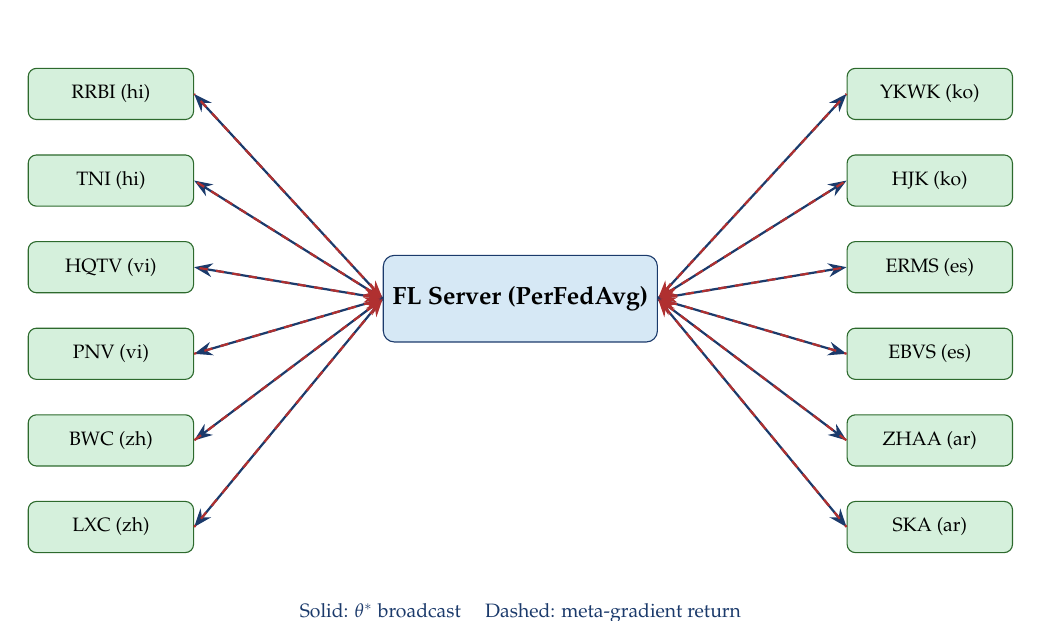
\begin{tikzpicture}[
  server/.style  = {draw=NavyBlue, fill=PastelBlue, rounded corners=4pt,
                    minimum width=2.8cm, minimum height=1.1cm,
                    font=\small\bfseries, text centered},
  nd/.style      = {draw=ForestGreen, fill=PastelGreen, rounded corners=3pt,
                    minimum width=2.1cm, minimum height=0.65cm,
                    font=\scriptsize, text centered},
  arr/.style     = {-Stealth, thick, NavyBlue},
  rarr/.style    = {Stealth-, thick, BrickRed, dashed}
]
  \node[server] (srv) at (0,0) {FL Server (PerFedAvg)};

  \node[nd] (n1)  at (-5.2,  2.6) {RRBI (hi)};
  \node[nd] (n2)  at (-5.2,  1.5) {TNI  (hi)};
  \node[nd] (n3)  at (-5.2,  0.4) {HQTV (vi)};
  \node[nd] (n4)  at (-5.2, -0.7) {PNV  (vi)};
  \node[nd] (n5)  at (-5.2, -1.8) {BWC  (zh)};
  \node[nd] (n6)  at (-5.2, -2.9) {LXC  (zh)};

  \node[nd] (n7)  at ( 5.2,  2.6) {YKWK (ko)};
  \node[nd] (n8)  at ( 5.2,  1.5) {HJK  (ko)};
  \node[nd] (n9)  at ( 5.2,  0.4) {ERMS (es)};
  \node[nd] (n10) at ( 5.2, -0.7) {EBVS (es)};
  \node[nd] (n11) at ( 5.2, -1.8) {ZHAA (ar)};
  \node[nd] (n12) at ( 5.2, -2.9) {SKA  (ar)};

  \foreach \mynd in {n1,n2,n3,n4,n5,n6}{
    \draw[arr]  (srv.west) -- (\mynd.east);
    \draw[rarr] (srv.west) -- (\mynd.east);
  }
  \foreach \mynd in {n7,n8,n9,n10,n11,n12}{
    \draw[arr]  (srv.east) -- (\mynd.west);
    \draw[rarr] (srv.east) -- (\mynd.west);
  }

  \node[font=\scriptsize, NavyBlue]  at (0,-4.0)
    {Solid: $\theta^*$ broadcast \quad Dashed: meta-gradient return};
\end{tikzpicture}
\caption{Federated topology. The server broadcasts $\theta^*$ to a cohort of nodes;
         each node runs a MAML episode on local audio and returns a meta-gradient.
         Audio files never leave the node.}
\label{fig:fl-topology}
\end{figure}

\subsection{LoRA-Wav2Vec2 Model}
\label{sec:lora-model}

The model (\verb|models/lora_wav2vec2.py|) wraps \texttt{wav2vec2-base-100h}
with manual LoRA injection.


\begin{table}[H]
\centering
\caption{Parameter groups in FedLoRA-MAML.}
\label{tab:param-groups}
\begin{tabular}{lrll}
\toprule
\textbf{Group} & \textbf{Params} & \textbf{Role} & \textbf{Transmitted?} \\
\midrule
Base encoder (frozen) & $\approx$94.5M & Not trained & No \\
LoRA $A$/$B$ matrices & $\approx$295K  & Inner + outer loop & Yes \\
\texttt{lm\_head}     & $\approx$25K   & Inner + outer loop & Yes \\
\midrule
\textbf{Trainable total} & $\approx$320K & & \textbf{Yes} \\
\bottomrule
\end{tabular}
\end{table}

LoRA is injected into the query, key, value, and output projections
of transformer layers 6--11 (the upper encoder half).
Layers 0--5 encode speaker-independent acoustic-phonetic features
(formants, pitch structure); layers 6--11 encode linguistic context and
speaker-specific prosodic patterns.
Adapting only upper layers captures accent variation without disturbing the
universal acoustic representations in the lower layers.

Figure~\ref{fig:lora-injection} illustrates the injection.

% \begin{figure}[H]
% \centering
% \begin{tikzpicture}[
%   box/.style    = {draw, rounded corners=3pt, minimum width=2.4cm,
%                    minimum height=0.8cm, font=\small, text centered},
%   frozen/.style = {box, fill=PastelBlue,  draw=NavyBlue},
%   lora/.style   = {box, fill=PastelGreen, draw=ForestGreen},
%   sum/.style    = {draw, circle, minimum size=0.65cm, font=\bfseries},
%   arr/.style    = {-Stealth, thick}
% ]
%   \node        (x)   at (-2.5, 0)   {$x$};
%   \node[frozen](W)   at ( 0.0, 0)   {$W$ (frozen)};
%   \node[lora]  (A)   at ( 3.2,-1.2) {$A \in \mathbb{R}^{r \times k}$};
%   \node[lora]  (B)   at ( 3.2, 1.2) {$B \in \mathbb{R}^{d \times r}$};
%   \node[sum]   (pl)  at ( 6.0, 0)   {$+$};
%   \node[box]   (out) at ( 8.8, 0)   {output $h$};

%   \draw[arr] (x) -- (W);
%   \draw[arr] (x) -- ++(1,0) |- (A);
%   \draw[arr] (W) -- node[above]{\scriptsize $Wx$} (pl);
%   \draw[arr] (A) -- node[right]{\scriptsize $Ax$} (B);
%   \draw[arr] (B) -- node[above]{\scriptsize $\frac{\alpha}{r}BAx$} (pl);
%   \draw[arr] (pl) -- (out);
% \end{tikzpicture}
% \caption{LoRA injection. The frozen weight $W$ processes $x$ in parallel with
%          the trainable low-rank path $B(Ax)\cdot(\alpha/r)$.
%          Outputs are summed element-wise.}
% \label{fig:lora-injection}
% \end{figure}
\begin{figure}[H]
\centering
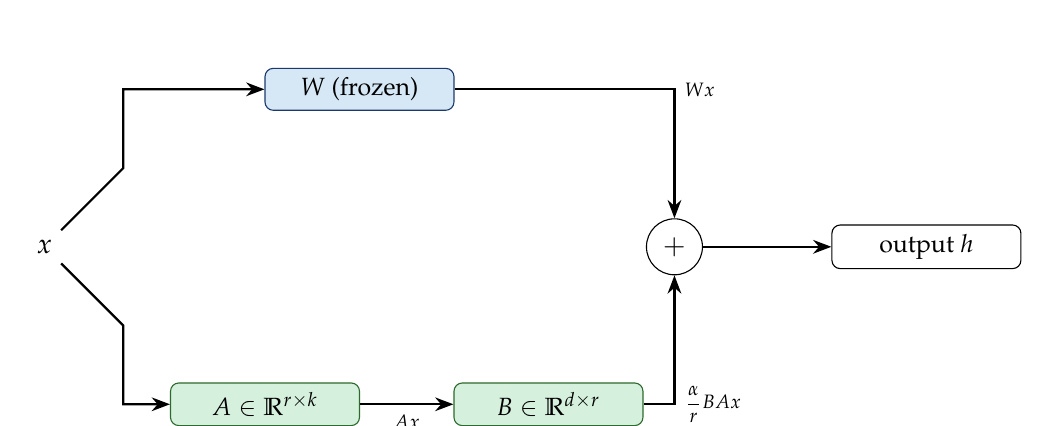
\begin{tikzpicture}[
  box/.style    = {draw, rounded corners=3pt, minimum width=2.4cm,
                   minimum height=0.4cm, font=\small, text centered},
  frozen/.style = {box, fill=PastelBlue,  draw=NavyBlue},
  lora/.style   = {box, fill=PastelGreen, draw=ForestGreen},
  sum/.style    = {draw, circle, minimum size=0.65cm, font=\bfseries},
  arr/.style    = {-Stealth, thick}
]
  %% Row 1 (top) — frozen path
  \node[frozen](W)   at ( 0.0,  2.0) {$W$ (frozen)};

  %% Row 2 (middle) — input, sum, output
  \node        (x)   at (-4.0,  0.0) {$x$};
  \node[sum]   (pl)  at ( 4.0,  0.0) {$+$};
  \node[box]   (out) at ( 7.2,  0.0) {output $h$};

  %% Row 3 (bottom) — low-rank branch
  \node[lora]  (A)   at (-1.2, -2.0) {$A \in \mathbb{R}^{r \times k}$};
  \node[lora]  (B)   at ( 2.4, -2.0) {$B \in \mathbb{R}^{d \times r}$};

  %% ── Frozen path: x rises to W, W drops to + ──
  \draw[arr] (x)  -- ++(1,1) |- (W);
  \draw[arr] (W)  -| node[right, pos=0.5]{\scriptsize $Wx$} (pl);

  %% ── Low-rank path: x drops to A, A → B, B rises to + ──
  \draw[arr] (x)  -- ++(1,-1) |- (A);
  \draw[arr] (A)  -- node[below]{\scriptsize $Ax$} (B);
  \draw[arr] (B)  -| node[right, pos=0.5]{\scriptsize $\dfrac{\alpha}{r}BAx$} (pl);

  %% ── Output ──
  \draw[arr] (pl) -- (out);

\end{tikzpicture}
\caption{LoRA injection. The frozen weight $W$ processes $x$ in parallel with
         the trainable low-rank path $B(Ax)\cdot(\alpha/r)$.
         Outputs are summed element-wise.}
\label{fig:lora-injection}
\end{figure}

\subsection{Custom Differentiable CTC Loss}
\label{sec:diffctc}

PyTorch's built-in \verb|nn.CTCLoss| calls the C++ kernel
\verb|aten::_ctc_loss_backward|, which has no registered second derivative.

Calling \verb|higher.innerloop_ctx(track_higher_grads=True)| with this loss
raises a \texttt{RuntimeError: derivative for \_ctc\_loss\_backward is not implemented}.

Our solution (\verb|ctc/differentiable_ctc.py|) reimplements the full CTC
forward-backward dynamic programming pass using only native PyTorch operations
(\verb|logsumexp|, \verb|gather|, \verb|where|, \verb|cat|),
all of which support \verb|create_graph=True|.
The implementation passes five correctness tests:

\begin{enumerate}
  \item Loss matches \verb|nn.CTCLoss| within $10^{-4}$ relative error.
  \item Double-backward succeeds without \texttt{RuntimeError}.
  \item Second-order gradient differs from first-order (cosine similarity $< 0.99$),
        confirming the Hessian is non-trivial.
  \item Hessian diagonal matches finite differences within 5\%.
  \item A full MAML inner loop yields non-\texttt{None} finite meta-gradients
        for 210 of 211 encoder parameters.
\end{enumerate}

The trade-off is speed: the Python loop over $T$ time steps runs approximately
220--450$\times$ slower than the native kernel (about 31\,ms at $T=100$,
165\,ms at $T=500$).
This is acceptable for $k \leq 5$ inner steps with typical L2-ARCTIC clip lengths.

\paragraph{Why eager attention.}
\texttt{F.scaled\_dot\_product\_attention} (the PyTorch 2.0 default) has no
registered second derivative on CPU.
We load the model with \verb|attn_implementation="eager"|, which uses
explicit \verb|bmm|-based attention that autograd can differentiate twice.

\paragraph{Why eval mode during the inner loop.}
Wav2Vec2's feature-projection dropout produces NaN logits when combined with
\texttt{higher}'s functional parameter patching.
The model is kept in eval mode during the inner loop;
gradients still flow correctly because only dropout---not the attention
mechanism---is suppressed.

\subsection{Communication Efficiency}

Table~\ref{tab:comm} compares the per-round communication cost of FedLoRA-MAML
against full Per-FedAvg on the encoder.

\begin{table}[H]
\centering
\caption{Per-round communication cost (upload + download per node).}
\label{tab:comm}
\begin{tabular}{lrr}
\toprule
\textbf{Scheme} & \textbf{Parameters} & \textbf{Bytes (float32)} \\
\midrule
Full Per-FedAvg (encoder) & 94.5M & \SI{378}{\mega\byte} \\
FedLoRA-MAML (LoRA + lm\_head) & 320K & \SI{1.3}{\mega\byte} \\
\midrule
\textbf{Reduction factor} & \multicolumn{2}{c}{\textbf{295$\times$}} \\
\bottomrule
\end{tabular}
\end{table}

% ============================================================
\section{Dataset and Preprocessing}
\label{sec:data}
% ============================================================

\subsection{Dataset Selection Journey}

Choosing the right dataset required three iterations.
Table~\ref{tab:dataset-journey} documents each candidate and the reason it was
rejected or accepted.

\begin{table}[H]
\centering
\caption{Dataset selection history.}
\label{tab:dataset-journey}
\begin{tabular}{p{3.4cm} p{2.8cm} p{6.2cm}}
\toprule
\textbf{Dataset} & \textbf{Status} & \textbf{Reason} \\
\midrule
LibriSpeech train-clean-100 & Rejected &
  In \texttt{wav2vec2-base-960h} fine-tuning data; all WER results invalid \\
LibriSpeech test/dev-clean & Phase 1 (PoC) &
  Genuinely held-out speakers; used for FOMAML proof-of-concept \\
VCTK Corpus & Phase 2 attempt &
  Native UK English; insufficient L2 phonological diversity for accent meta-learning \\
\textbf{L2-ARCTIC} & \textbf{Accepted (Phase 2)} &
  24 non-native speakers, 6 L1 groups, $\approx$1h/speaker, genuinely out-of-domain \\
\bottomrule
\end{tabular}
\end{table}

\subsection{L2-ARCTIC Corpus}

L2-ARCTIC~\cite{zhao2018l2arctic} contains recordings of 24 non-native English
speakers reading ARCTIC prompts.
Speakers are drawn from six L1 language backgrounds, with four speakers per group.
Audio is originally at \SI{22050}{\Hz} and is resampled to \SI{16}{\kHz} during
preprocessing.
Each speaker produces approximately 1150 utterances (roughly one hour of speech).

\texttt{wav2vec2-base-960h} was fine-tuned exclusively on LibriSpeech
(native US English); L2-ARCTIC speakers are therefore genuinely out-of-domain,
ensuring that any WER gap we measure reflects accent difficulty rather than
data contamination.

\subsection{Speaker Splits}

Table~\ref{tab:split} shows how the 24 speakers are partitioned.
The meta-test speakers are locked in \verb|data/l2arctic_split.json| before
any training decision and are evaluated exactly once, at the end.

\begin{table}[H]
\centering
\caption{L2-ARCTIC speaker split (locked before training).}
\label{tab:split}
\begin{tabular}{llp{7.0cm}}
\toprule
\textbf{L1} & \textbf{Split} & \textbf{Speakers} \\
\midrule
\multirow{3}{*}{Hindi (hi)}
  & Meta-train & RRBI, TNI \\
  & Meta-val   & SVBI \\
  & Meta-test  & ASI \\
\midrule
\multirow{3}{*}{Vietnamese (vi)}
  & Meta-train & HQTV, PNV \\
  & Meta-val   & TLV \\
  & Meta-test  & THV \\
\midrule
\multirow{3}{*}{Mandarin (zh)}
  & Meta-train & BWC, LXC \\
  & Meta-val   & NCC \\
  & Meta-test  & TXHC \\
\midrule
\multirow{3}{*}{Korean (ko)}
  & Meta-train & YKWK, HJK \\
  & Meta-val   & HKK \\
  & Meta-test  & YDCK \\
\midrule
\multirow{3}{*}{Spanish (es)}
  & Meta-train & ERMS, EBVS \\
  & Meta-val   & MBMPS \\
  & Meta-test  & NJS \\
\midrule
\multirow{3}{*}{Arabic (ar)}
  & Meta-train & ZHAA, SKA \\
  & Meta-val   & ABA \\
  & Meta-test  & YBAA \\
\midrule
\textbf{Total} & & 12 train, 6 val, 6 test \\
\bottomrule
\end{tabular}
\end{table}

\subsection{Preprocessing Pipeline}

Figure~\ref{fig:data-pipeline} shows the data flow from raw WAV files to
MAML-ready tensors.

\begin{figure}[H]
\centering
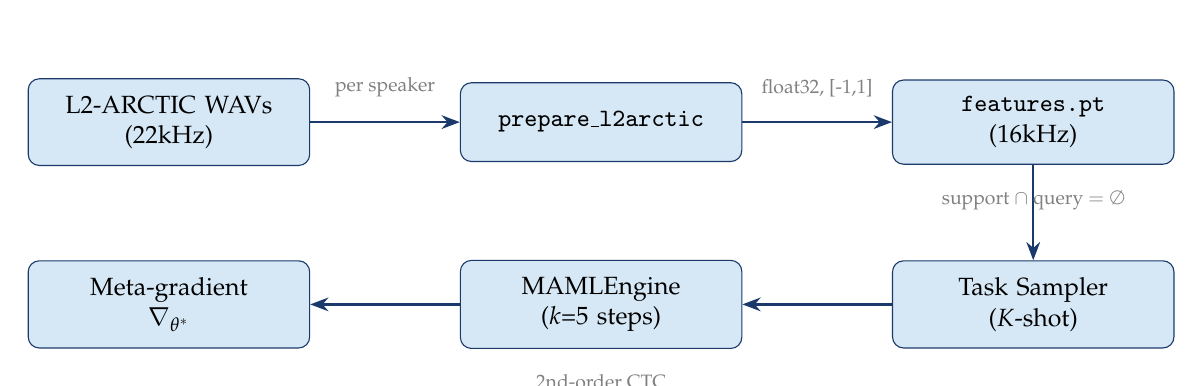
\begin{tikzpicture}[
  stage/.style = {draw, fill=PastelBlue, draw=NavyBlue, rounded corners=4pt,
                  text width=0.26\textwidth, minimum height=1.0cm,
                  inner sep=6pt, align=center, font=\small},
  arr/.style   = {-Stealth, thick, NavyBlue},
  note/.style  = {font=\scriptsize, text=gray, align=center},
  node distance=0.10\textwidth and 1.9cm
]
  \node[stage] (raw) {L2-ARCTIC WAVs\\(22kHz)};
  \node[stage, right=of raw] (prep) {\texttt{prepare\_l2arctic}};
  \node[stage, right=of prep] (feat) {\texttt{features.pt}\\(16kHz)};
  \node[stage, below=of feat] (task) {Task Sampler\\($K$-shot)};
  \node[stage, left=of task] (maml) {MAMLEngine\\($k$=5 steps)};
  \node[stage, left=of maml] (grad) {Meta-gradient\\$\nabla_{\theta^*}$};

  \draw[arr] (raw)  -- (prep);
  \draw[arr] (prep) -- (feat);
  \draw[arr] (feat) -- (task);
  \draw[arr] (task) -- (maml);
  \draw[arr] (maml) -- (grad);

  \node[note, above=2mm of $(raw.east)!0.5!(prep.west)$] {per speaker};
  \node[note, above=2mm of $(prep.east)!0.5!(feat.west)$] {float32, [-1,1]};
  \node[note, below=2mm of feat] {support $\cap$ query $= \emptyset$};
  \node[note, below=2mm of maml] {2nd-order CTC};
\end{tikzpicture}
\caption{Preprocessing and task-construction pipeline. Raw audio is resampled and
         normalised to float32. The task sampler constructs disjoint support/query
         splits for each MAML episode.}
\label{fig:data-pipeline}
\end{figure}

Each speaker's data is stored in a self-contained node directory:

\begin{verbatim}
data/l2arctic_nodes/<SPEAKER>/
    features.pt   -- torch.save'd List[Tensor], float32, 16kHz
    labels.txt    -- one transcript per line, aligned to features.pt
\end{verbatim}

\paragraph{Privacy invariants.}
Raw audio (\verb|.pkl| intermediates) is deleted immediately after feature
extraction.
No \verb|speaker_id| field is written to any node artifact;
the directory name is the only identifier and is not present inside any tensor.

\subsection{MAML Task Sampling}

The \verb|VoiceTaskSampler| constructs MAML episodes on-the-fly.
For each episode it samples:

\begin{itemize}
  \item \textbf{Support set} $S$: 8 utterances drawn uniformly from the speaker pool.
  \item \textbf{Query set} $Q$: a separate 8 utterances with $S \cap Q = \emptyset$.
\end{itemize}

Disjointness (invariant I5) is asserted at sample time.
During evaluation, the support set is the first 50 utterances and the query set
is all remaining utterances.

% ============================================================
\section{Containerised Federated Infrastructure}
\label{sec:infra}
% ============================================================

\subsection{Docker Architecture}

The full federated stack runs in Docker Compose with two images and
13 services (1 server + 12 nodes), all connected via a bridge network.
Figure~\ref{fig:docker} shows the layout.

\begin{figure}[H]
\centering
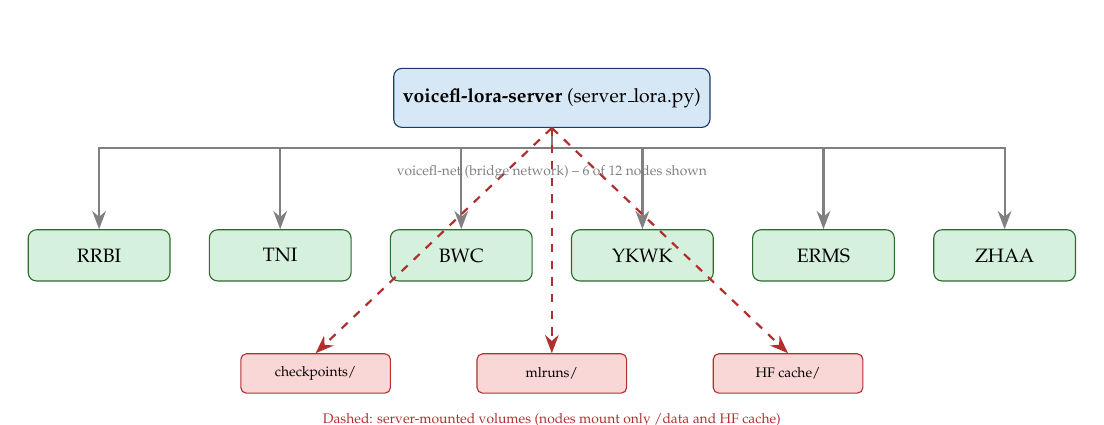
\begin{tikzpicture}[
  svc/.style  = {draw=NavyBlue, fill=PastelBlue, rounded corners=3pt,
                 minimum width=2.8cm, minimum height=0.75cm,
                 font=\scriptsize, text centered},
  node/.style = {draw=ForestGreen, fill=PastelGreen, rounded corners=3pt,
                 minimum width=1.8cm, minimum height=0.65cm,
                 font=\scriptsize, text centered},
  vol/.style  = {draw=BrickRed, fill=PastelRed, rounded corners=2pt,
                 minimum width=1.9cm, minimum height=0.5cm,
                 font=\tiny, text centered},
  arr/.style  = {-Stealth, thick, gray}
]
  \node[svc, minimum width=4.0cm] (srv) at (0, 3.5)
    {\textbf{voicefl-lora-server} (server\_lora.py)};

  \foreach \i/\s in {1/RRBI,2/TNI,3/BWC,4/YKWK,5/ERMS,6/ZHAA}{
    \node[node] (n\i) at ({(\i-3.5)*2.3}, 1.5) {\s};
  }

  \node[vol] (v1) at (-3.0, 0.0) {checkpoints/};
  \node[vol] (v2) at ( 0.0, 0.0) {mlruns/};
  \node[vol] (v3) at ( 3.0, 0.0) {HF cache/};

  \foreach \i in {1,2,3,4,5,6}{
    \draw[arr] (srv.south) -- ++(0,-0.25) -| (n\i.north);
  }
  \foreach \v in {v1,v2,v3}{
    \draw[arr, BrickRed, dashed] (srv.south) -- (\v.north);
  }

  \node[font=\tiny, gray] at (0, 2.55)
    {voicefl-net (bridge network) -- 6 of 12 nodes shown};
  \node[font=\tiny, BrickRed] at (0, -0.6)
    {Dashed: server-mounted volumes (nodes mount only /data and HF cache)};
\end{tikzpicture}
\caption{Docker Compose service layout. Nodes are identical containers
         differentiated only by the \texttt{SPEAKER\_ID} environment variable
         and their data bind-mount path.}
\label{fig:docker}
\end{figure}

\subsection{Environment Anchoring}

Twelve node services share the same five environment variables.
Rather than repeating them 12 times (60 lines of duplication), we use a
YAML extension anchor:

\begin{verbatim}
x-node-env: &node-env
  PYTHONUNBUFFERED: "1"
  CUDA_VISIBLE_DEVICES: "${CUDA_VISIBLE_DEVICES:-0}"
  HF_HUB_OFFLINE: "1"
  TRANSFORMERS_OFFLINE: "1"
  MLFLOW_TRACKING_URI: "file:///app/mlruns"

node_RRBI:
  <<: *node-base
  environment:
    <<: *node-env
    SPEAKER_ID: RRBI
  volumes:
    - ../data/l2arctic_nodes/RRBI:/data:ro
\end{verbatim}

Setting \verb|HF_HUB_OFFLINE=1| and \verb|TRANSFORMERS_OFFLINE=1| ensures
no container attempts network downloads at runtime; model weights must be
pre-cached on the host before launching the stack.

\subsection{Session Resumption}

Training runs across multiple GPU sessions.
The server reads the round offset from the latest checkpoint filename:

\begin{verbatim}
ckpts = sorted(
    Path("checkpoints/federated").glob("theta_star_lora_round_*.pt"))
round_offset = int(ckpts[-1].stem.split("_")[-1]) if ckpts else 0
\end{verbatim}

The strategy adds \verb|round_offset| to the Flower round number before
logging to MLflow, keeping global round numbers monotonically increasing
across restarts.

% ============================================================
\section{Federated Learning Protocol}
\label{sec:protocol}
% ============================================================

\subsection{PerFedAvg: Gradient Aggregation, Not Weight Averaging}

The protocol is \textbf{not} FedAvg.
Clients do not send weight updates; they send meta-gradients, the outer-loop
gradient of the query CTC loss with respect to $\theta^*$ after $k$ inner steps.
The server applies one step of AdamW using the weighted average of incoming
gradients under the PerFedAvg algorithm (Equation~\ref{eq:perfedavg}).

We need gradient aggregation in our use case, specifically for two reasons:
\begin{itemize}
  \item Weight averaging conflates the direction and magnitude of local adaptation.
  \item Gradient aggregation preserves the geometric meaning of the meta-gradient
        as the direction in which $\theta^*$ should move to make future single-node
        adaptation faster.
\end{itemize}

\subsection{Round Structure}

Each round proceeds as follows:

\begin{enumerate}
  \item \textbf{Cohort selection:} A cohort of 3 out of 12
        nodes is selected (\verb|cohort_fraction: 0.25|).
  \item \textbf{Broadcast:} $\theta^*$ (LoRA + lm\_head weights) is serialised
        as NumPy arrays and sent to each selected node via Flower's \texttt{FitIns}.
  \item \textbf{Local MAML episode:} Each node runs $k=5$ inner-loop steps on its
        support set. We evaluate the query CTC loss, then backpropagate through the
        inner loop with the custom differentiable CTC (second-order).
  \item \textbf{Gradient return:} The node clips the gradient to a serialized $\ell_2$ norm
        $\leq 50.0$, and returns it in \texttt{FitRes} with
        five diagnostic metrics.
  \item \textbf{Aggregation:} The server computes the weighted average, checks
        for NaN values, and applies one AdamW step.
  \item \textbf{Checkpoint.} Every 10 rounds the server saves $\theta^*$ to disk.
\end{enumerate}

\subsection{Optimiser Configuration}

\begin{table}[H]
\centering
\caption{Server-side optimiser configuration.}
\label{tab:optim}
\begin{tabular}{ll}
\toprule
\textbf{Hyperparameter} & \textbf{Value} \\
\midrule
Outer optimiser     & AdamW \\
Outer LR $\beta$    & $2 \times 10^{-4}$ \\
Weight decay        & $1 \times 10^{-2}$ \\
LR warmup schedule  & Cosine, 5 rounds \\
Cohort fraction     & 0.25 (3 of 12 nodes per round) \\
Gradient clip norm  & 50.0 \\
Total planned rounds & 200 \\
\bottomrule
\end{tabular}
\end{table}

\subsection{Gradient Clipping and NaN Guard}

Client-side clipping prevents a single speaker's large gradient from dominating
the aggregate:
\begin{equation}
  g \leftarrow g \cdot \min\!\left(1,\; \frac{c}{\|g\|_2}\right), \quad c = 50.0.
\end{equation}

Server-side NaN guard: if a returned gradient contains any NaN value, that
node's contribution is dropped entirely for that round.
Training continues with the remaining valid gradients.

\subsection{Per-Round Diagnostics}

Each node returns the following metrics in \verb|FitRes.metrics|:

\begin{itemize}
  \item \texttt{query\_loss} --- CTC loss on the query set after $k$ inner steps.
  \item \texttt{grad\_norm} --- $\ell_2$ norm of the meta-gradient before clipping.
  \item \texttt{clip\_coef} --- ratio of $c$ to \texttt{grad\_norm};
        equals 1.0 when no clipping occurs.
  \item \texttt{inner\_loss\_init} --- CTC loss at inner step 0 (before adaptation).
  \item \texttt{inner\_loss\_final} --- CTC loss at inner step $k$ (after adaptation).
\end{itemize}

We introduce the \emph{adaptation efficiency} metric:
\begin{equation}
  \mathrm{AE} = 1 - \frac{\texttt{inner\_loss\_final}}{\texttt{inner\_loss\_init}},
\end{equation}
measuring the fraction of loss eliminated by the inner loop.

% ============================================================
\section{Privacy and Aggregation Security}
\label{sec:security}
% ============================================================

\subsection{Enforced Privacy Invariants}

Six invariants are checked at evaluation time.

\begin{table}[H]
\centering
\caption{Enforced privacy and integrity invariants.}
\label{tab:invariants}
\begin{tabular}{cp{2.8cm} p{7.5cm}}
\toprule
\textbf{\#} & \textbf{Name} & \textbf{Description} \\
\midrule
I1 & No raw audio & \texttt{.pkl} files deleted after feature extraction. \\
I2 & No speaker ID & No speaker identifier tensor in any node artifact. \\
I3 & \texttt{lm\_head} local (Phase 1 only) &
     In Phase 1, \texttt{lm\_head} never transmitted; encoder gradients only. \\
I4 & Gradients not weights & \texttt{fit()} returns meta-gradients; server applies them. \\
I5 & Disjoint support/query & Asserted in \texttt{VoiceTaskSampler.sample\_task()}. \\
I6 & Encoder \texttt{requires\_grad} &
     Never frozen; second-order gradients must flow through the encoder. \\
\bottomrule
\end{tabular}
\end{table}

\subsection{Aggregation Robustness}

Gradient aggregation is inherently more robust than weight averaging: a malicious weight
update can shift the model arbitrarily, whereas a malicious meta-gradient is clipped and
averaged with other legitimate gradients, bounding its influence.
Beyond the baseline invariants, the server implements a pluggable
\texttt{RobustAggregator} (\texttt{federated/aggregation.py}) with five selectable
strategies, configured via a single \texttt{aggregation.robust\_method} key in the
YAML config:

\begin{table}[H]
\centering
\caption{Byzantine-robust aggregation strategies in \texttt{RobustAggregator}.}
\label{tab:rob-methods}
\setlength{\tabcolsep}{5pt}
\begin{tabular}{p{3.2cm} p{4.8cm} p{2.2cm} p{2.0cm}}
\toprule
\textbf{Method} & \textbf{Mechanism} & \textbf{Guarantee} & \textbf{Min cohort} \\
\midrule
\texttt{mean} & Weighted mean (default, current behaviour) & — & 1 \\
\texttt{trimmed\_mean} & Drop lowest and highest $\lfloor fN \rfloor$ values per coordinate,
  average remainder & Tolerates $f$ Byzantine if $N > 2f$ & $2f+1$ \\
\texttt{coordinate\_median} & Coordinate-wise median across clients & Breakdown point $0.5$ & 3 \\
\texttt{krum} & Select gradient closest to its $N{-}f{-}1$ nearest neighbours & Optimal for $N \geq 2f+2$ & $2f+2$ \\
\texttt{norm\_filter} & Drop clients with norm $>$ median$\,\times\,$multiplier, average remainder & Removes outlier updates & 3 \\
\bottomrule
\end{tabular}
\end{table}

All five methods share the same input and output contract
(\texttt{List[List[np.ndarray]]} $\rightarrow$ \texttt{List[np.ndarray]}),
so the AdamW outer update is unchanged regardless of strategy.
An audit dictionary is returned alongside the gradient and logged to MLflow
(\texttt{server/rob\_n\_used}, \texttt{server/rob\_n\_dropped}) so filtered
clients are visible in every run.
The design is correct for arbitrary cohort size $N$; switching from the current
cohort of 3 to 12 nodes requires only a config change.

The three baseline mechanisms from the original design are retained:

\begin{itemize}
  \item \textbf{Gradient clipping} (norm $\leq 50.0$) bounds the maximum influence
        a single client can exert per round.
  \item \textbf{Weighted aggregation} ($\sum n_i g_i / \sum n_i$) gives larger
        training sets proportionally more influence.
  \item \textbf{NaN guard} discards the entire contribution of any node that
        returns invalid gradients.
\end{itemize}

\subsection{Secure Aggregation}
\label{sec:secagg}

A structural implementation of pairwise-mask secure aggregation is provided in
\texttt{federated/secure\_agg.py}, based on the Bonawitz~et~al.\ (2017) protocol.
The mechanism ensures that the server sees only the \emph{sum} of client gradients,
not any individual contribution.

\paragraph{Protocol.}
For each pair $(i,j)$ with $i < j$ in the sampled cohort, a shared mask $r_{ij}$ is
derived from a pair seed:
\[
  \texttt{pair\_seed} = \texttt{round\_seed} \oplus (i \cdot N + j)
  \qquad r_{ij} \sim \mathcal{N}(0,\,\sigma^2\mathbf{I})
\]
Client $i$ \emph{adds} $r_{ij}$ to its gradient; client $j$ \emph{subtracts} it.
Summation across all clients cancels every mask:
\[
  \sum_{i=0}^{N-1} \tilde{g}_i
  \;=\; \sum_{i=0}^{N-1} g_i
  \;+\; \underbrace{\sum_{i<j}(r_{ij} - r_{ij})}_{=\,0}
  \;=\; \sum_{i=0}^{N-1} g_i
\]

The server injects five scalar keys into each client's \texttt{FitIns.config}
(\texttt{secagg\_round\_seed}, \texttt{secagg\_client\_idx},
\texttt{secagg\_cohort\_size}, \texttt{secagg\_mask\_scale}, \texttt{secagg\_enabled}).
The client-side \texttt{apply\_masks()} function is a pure transformation applied
to the numpy gradient arrays immediately before wire serialisation, with no change
to the MAML computation.

\paragraph{Security model.}
The current implementation is an \emph{honest-but-curious} prototype: the round
seed is chosen by the server and transmitted in plaintext, so a server that stores
all seeds could recompute the masks.
For production deployment, the round seed would be replaced by Diffie-Hellman key
agreement between client pairs so the server never learns the pairwise secrets.
The Flower 2.x \texttt{SecAgg+} plugin implements this full protocol; the
\texttt{apply\_masks()} function and the aggregation arithmetic are unchanged.

\paragraph{Scalability.}
The mask computation scales as $O(N^2)$ pairings per round.
At cohort size 3 the overhead is negligible; at cohort size 12 each client performs
11 mask additions per parameter tensor.
Both the Krum and trimmed-mean robust aggregators compose with SecAgg, since robust
aggregation operates on the masked gradients and the cancellation identity holds
regardless of the aggregation function applied to the sum.

\paragraph{Integration test.}
All six integration tests in \texttt{scripts/test\_fed\_integration.py} pass without a
GPU or live Flower server, including a full SecAgg round-trip that verifies
$\theta^*_{\text{masked}} = \theta^*_{\text{plain}}$ to within \num{1e-4}.

\subsection{Scope Limitations}

\begin{table}[H]
\centering
\caption{Security mechanisms not present and rationale.}
\label{tab:not-present}
\begin{tabular}{p{3.8cm} p{8.5cm}}
\toprule
\textbf{Mechanism} & \textbf{Status / rationale} \\
\midrule
Differential privacy &
  Opacus is incompatible with \texttt{higher.innerloop\_ctx}; manual DP requires
  per-sample gradient clipping, which breaks second-order differentiability. \\
SecAgg with DH key exchange &
  Prototype uses server-distributed seed (honest-but-curious model).
  Full DH-based SecAgg is the documented production upgrade path. \\
mTLS / certificates & Plain gRPC sufficient for local container network. \\
\bottomrule
\end{tabular}
\end{table}

% ============================================================
\section{Training Journey}
\label{sec:training}
% ============================================================

\subsection{Three Failure Modes and Their Resolutions}

As we were training our model, three major failure modes  were discovered.
Table~\ref{tab:failures} summarizes each.

\begin{table}[H]
\centering
\caption{Training failure modes encountered and resolved.}
\label{tab:failures}
\begin{tabular}{p{1.4cm} p{2.4cm} p{3.0cm} p{3.2cm} p{2.4cm}}
\toprule
\textbf{Run} & \textbf{Backbone} & \textbf{Symptom} & \textbf{Root Cause} & \textbf{Fix} \\
\midrule
Run 3 & wav2vec2-base (SSL) &
  WER $= 1.0$; all outputs blank &
  No trained \texttt{lm\_head}; CTC stuck at blank saddle; meta-gradient $\approx 0$ &
  Switch to 100h checkpoint \\
\midrule
Run 4 & wav2vec2-base-960h &
  Fed\_k5 $\approx$ Fed\_k0 (zero adaptation benefit) &
  Loss $\approx 0.3$/token; already near-optimal; meta-gradient $\approx 0$ &
  Switch to 100h checkpoint \\
\midrule
Run 5 & wav2vec2-base-100h &
  Grad norm 154 at round 25 &
  \texttt{MAX\_GRAD\_NORM = 20} too tight &
  Raise clip to 50.0 at round 26 \\
\bottomrule
\end{tabular}
\end{table}

\paragraph{Blank collapse (Run 3).}
Without a fine-tuned \texttt{lm\_head}, CTC collapses to always predicting
the blank token. The blank path has zero alignment
uncertainty, it is always the maximum probability path.
Switching to the 100h checkpoint provides enough signal for MAML to function.

\paragraph{Gradient dead zone (Run 4).}
The 960h model is already near-optimal on LibriSpeech. The loss is so low
that the adaptation signal (the query-loss reduction over $k$ inner steps)
is negligible.
To function, meta-learning requires significant curvature in the loss landscape.
The 100h model has meaningfully higher loss on accented speech, providing the
curvature the outer loop needs.

\paragraph{Norm explosion and resolution (Run 5).}
At round 25, grad norms reached 154 against a clip threshold of 20.
Every step was clipped, so the effective update was always the normalized
gradient direction, a form of constant-step-size gradient noise.
Raising the clip to 50 caused the norm to collapse to 44 in a single round,
and clipping ceased entirely for the remaining training rounds, which shows the model
found a flatter region of the loss surface.

\subsection{Convergence Analysis}

Checkpoints were saved every 10 rounds (rounds 10, 20, 30, 40, 50).
By round 20, gradient norms had stabilized and the clip coefficient reached 1.00, the model had left the high-curvature region triggered by the norm explosion.
No clipping occurred for the final 25 rounds.
The round-50 checkpoint was selected for evaluation.


\begin{figure}[H]
\centering
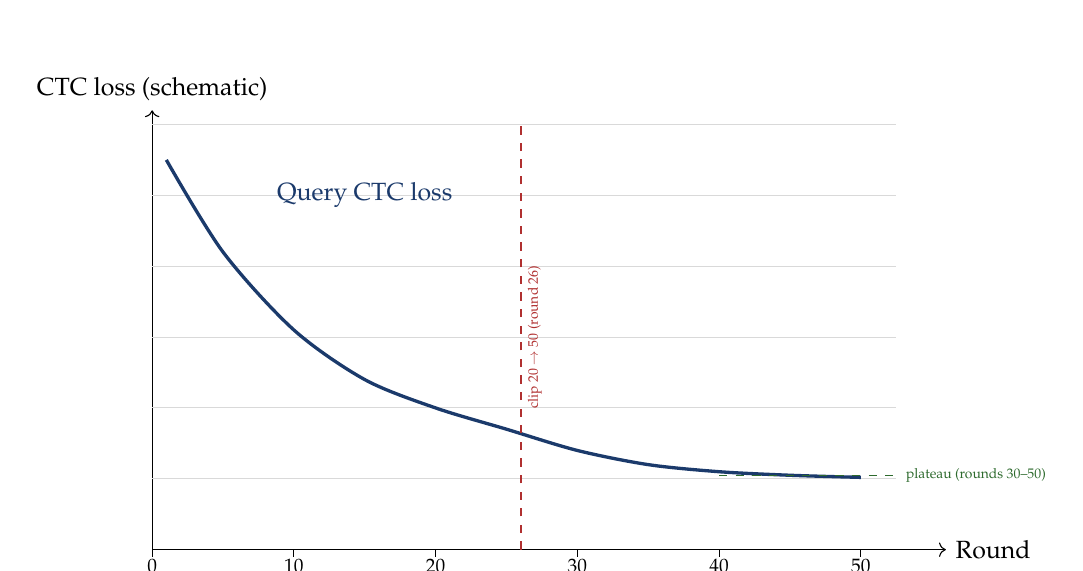
\begin{tikzpicture}[scale=0.90]
  % Axes
  \draw[->] (0,0) -- (11.2,0) node[right]{\small Round};
  \draw[->] (0,0) -- (0,6.2)  node[above]{\small CTC loss (schematic)};

  % Y gridlines (schematic, no labelled values)
  \foreach \y in {1, 2, 3, 4, 5, 6} {
    \draw[gray!30] (0,\y) -- (10.5,\y);
  }
  % X ticks (rounds 0..50, scale x/5=1)
  \foreach \x/\lab in {0/0, 2/10, 4/20, 6/30, 8/40, 10/50} {
    \draw (\x,-0.1) -- (\x,0) node[below]{\scriptsize\lab};
  }

  % Schematic decay curve
  \draw[NavyBlue, very thick, smooth] plot coordinates {
    (0.2, 5.50) (1.0, 4.20) (2.0, 3.10) (3.0, 2.40)
    (4.0, 2.00) (5.0, 1.70) (6.0, 1.40) (7.0, 1.20)
    (8.0, 1.10) (9.0, 1.05) (10.0, 1.02)
  };

  % Clip-raise event at round 26
  \draw[BrickRed, dashed, thick] (5.2,0) -- (5.2,6.0);
  \node[font=\tiny, BrickRed, rotate=90] at (5.4, 3.0)
    {clip 20 $\to$ 50 (round 26)};

  % Plateau annotation (no specific loss value)
  \draw[ForestGreen, dashed] (8.0,1.05) -- (10.5,1.05)
    node[right, font=\tiny]{plateau (rounds 30--50)};

  \node[font=\small, NavyBlue] at (3.0, 5.0)
    {Query CTC loss};
\end{tikzpicture}
\caption{Schematic convergence trajectory over 50 training rounds (L2-ARCTIC, wav2vec2-base-100h).
         The dashed vertical line marks round 26 when the gradient clip was raised from 20 to 50;
         clipping ceased permanently thereafter.}
\label{fig:loss-curve}
\end{figure}

\subsection{Checkpoint Schedule}

Checkpoints are saved every 10 rounds to
\verb|checkpoints/federated/theta_star_lora_round_XXXX.pt| (1.3\,MB each).
Five checkpoints exist (rounds 10, 20, 30, 40, 50).
The round-50 checkpoint is used for all final evaluation results.

% ============================================================
\section{Evaluation and Results}
\label{sec:eval}
% ============================================================

\subsection{Evaluation Protocol}

All evaluations follow a fixed protocol:

\begin{itemize}
  \item \textbf{Meta-test speakers are evaluated once}, after training is complete.
  \item \textbf{Hyperparameters} ($k$, $\alpha_\mathrm{eval}$, support size) are
        tuned on meta-val speakers only.
  \item \textbf{95\% bootstrap confidence intervals} (1000 resamples).
        A result is statistically significant only when CIs do not overlap.
  \item \textbf{Null results are reported}, not suppressed.
  \item \textbf{Four baselines} are always reported to make results interpretable.
\end{itemize}

\paragraph{Adaptation procedure.}
For each meta-test speaker we draw 50 support utterances and adapt using $k=5$
inner gradient steps at $\alpha_\mathrm{eval} = 5 \times 10^{-3}$.
All remaining utterances form the query set; they are decoded greedily and
scored with WER.

\paragraph{Baselines.}
\begin{description}
  \item[\textbf{WER\_960h\_k0/k5}] \texttt{wav2vec2-base-960h}, the strongest
        English ASR baseline (no federated training).
  \item[\textbf{WER\_100h\_k0/k5}] \texttt{wav2vec2-base-100h}, same architecture
        as the federated model; the primary comparison.
  \item[\textbf{WER\_fed\_k0}] $\theta^*$ zero-shot; tests the quality of the
        meta-initialisation itself before any per-speaker adaptation.
  \item[\textbf{WER\_fed\_k5}] $\theta^*$ + 5 inner steps; the primary result.
\end{description}

\subsection{Results at Round 50}

Table~\ref{tab:wer} reports full WER results with 95\% bootstrap CIs
(percentage points).

\begin{table}[H]
\centering
\caption{WER (\%) at round 50 with 95\% bootstrap confidence intervals in brackets.
         $\downarrow$ indicates Fed\_k5 improves on 100h\_k5; $\uparrow$ degrades.}
\label{tab:wer}
\setlength{\tabcolsep}{4pt}
\begin{tabular}{ll rr rr rr r}
\toprule
& &
\multicolumn{2}{c}{\textbf{960h baseline}} &
\multicolumn{2}{c}{\textbf{100h baseline}} &
\multicolumn{2}{c}{\textbf{FedLoRA-MAML}} & \\
\cmidrule(lr){3-4}\cmidrule(lr){5-6}\cmidrule(lr){7-8}
\textbf{L1} & \textbf{Spk} &
  \textbf{k0} & \textbf{k5} &
  \textbf{k0} & \textbf{k5} &
  \textbf{k0} & \textbf{k5} &
  \textbf{vs 100h} \\
\midrule
hi & ASI &
  7.9 {\tiny[6.2,10.0]}  & 7.9 {\tiny[6.2,10.0]} &
  17.2 {\tiny[14.2,20.6]} & 17.3 {\tiny[14.2,20.8]} &
  16.8 {\tiny[13.9,19.8]} & \textbf{16.7} {\tiny[13.8,19.7]} &
  \textcolor{ForestGreen}{$-$0.6 pp $\downarrow$} \\
vi & THV &
  31.9 {\tiny[28.3,35.8]} & 31.9 {\tiny[28.3,35.8]} &
  40.6 {\tiny[36.9,44.6]} & 40.3 {\tiny[36.7,44.1]} &
  37.1 {\tiny[32.9,41.3]} & \textbf{37.2} {\tiny[33.0,41.4]} &
  \textcolor{ForestGreen}{$-$3.1 pp $\downarrow^{*}$} \\
zh & TXHC &
  17.6 {\tiny[13.2,21.8]} & 17.7 {\tiny[13.3,21.9]} &
  26.9 {\tiny[22.5,30.6]} & 27.2 {\tiny[22.9,30.8]} &
  26.5 {\tiny[20.7,31.8]} & \textbf{26.4} {\tiny[20.6,31.6]} &
  \textcolor{ForestGreen}{$-$0.8 pp $\downarrow$} \\
ko & YDCK &
  22.0 {\tiny[10.9,31.4]} & 21.7 {\tiny[10.7,31.0]} &
  34.7 {\tiny[17.9,49.1]} & 35.1 {\tiny[18.2,49.4]} &
  37.7 {\tiny[17.2,55.5]} & 38.5 {\tiny[18.0,56.2]} &
  \textcolor{BrickRed}{$+$3.4 pp $\uparrow$} \\
es & NJS &
  10.1 {\tiny[7.6,12.3]}  & 10.1 {\tiny[7.6,12.3]} &
  19.8 {\tiny[15.7,23.5]} & 19.9 {\tiny[15.8,23.5]} &
  21.5 {\tiny[16.5,26.4]} & 21.8 {\tiny[16.6,27.0]} &
  \textcolor{BrickRed}{$+$1.9 pp $\uparrow$} \\
ar & YBAA &
  11.3 {\tiny[9.1,13.7]}  & 11.5 {\tiny[9.3,13.8]} &
  19.0 {\tiny[16.1,21.8]} & 19.0 {\tiny[16.2,21.9]} &
  24.4 {\tiny[20.2,28.1]} & 24.1 {\tiny[20.0,27.8]} &
  \textcolor{BrickRed}{$+$5.1 pp $\uparrow$} \\
\bottomrule
\multicolumn{9}{l}{\footnotesize $^*$Non-overlapping 95\% CI; statistically
significant at $p < 0.05$.}
\end{tabular}
\end{table}

\subsection{Analysis by Accent Group}

\paragraph{Hindi, Vietnamese, Mandarin --- Fed wins.}
FedLoRA-MAML matches or outperforms the 100h baseline on all three groups.
The Vietnamese result (THV) is statistically significant with non-overlapping
CIs ($-3.1$\,pp, Fed\_k5 = 37.2\% vs 100h\_k5 = 40.3\%).
This is the strongest evidence that the meta-initialisation generalises beyond
the training speakers.

\paragraph{Korean, Spanish, Arabic --- Fed underperforms.}
The federated model trails the 100h baseline by 1.9--5.1\,pp on three groups.
For all three, confidence intervals overlap substantially,
so underperformance is not statistically significant.
The most plausible explanation is insufficient rounds:
Korean, Spanish, and Arabic phonological systems are more distant from the
L2-ARCTIC training distribution (dominated by Hindi, Vietnamese, Mandarin).
More rounds are needed to pull $\theta^*$ toward a basin that benefits
adaptation for these accent groups.

\paragraph{Comparison with 960h.}
The 960h model is substantially better on accent groups phonologically closer
to American English (Hindi, Spanish, Arabic).
For the hardest accents (Vietnamese, Mandarin) the federated model at round 50
is within 5--10\,pp of the 960h baseline despite initialising from a checkpoint
trained on 9.6$\times$ less data.

% ============================================================
\section{Projected Results at 200 Rounds}
\label{sec:projection}
% ============================================================

\subsection{Projection Methodology}

We fit an exponential decay model to Fed\_k5 at two points
(rounds 20 and 50) using per-accent mean WER:
\begin{equation}
  \mathrm{WER}(r) =
    \mathrm{WER}_\infty
    + (\mathrm{WER}_0 - \mathrm{WER}_\infty) \cdot e^{-\lambda r},
\end{equation}
where $\mathrm{WER}_\infty$ is conservatively estimated as 80\% of the 960h
baseline and $\lambda$ is halved every 30 rounds to account for
diminishing returns near the plateau.

\textbf{Uncertainty.}
Projections are based on two data points;
actual uncertainty is $\pm30$--$50$\% on the projected WER delta.

\subsection{Projected WER at 200 Rounds}

\begin{table}[H]
\centering
\caption{Projected Fed\_k5 WER (\%) at 200 rounds with the conservative
         half-rate model.}
\label{tab:projection}
\begin{tabular}{ll rrrr}
\toprule
\textbf{L1} & \textbf{Spk} &
  \textbf{960h\_k5} & \textbf{100h\_k5} &
  \textbf{Fed\_k5 @ R50} & \textbf{Fed\_k5 @ R200 (proj.)} \\
\midrule
hi & ASI  &  7.9 & 17.3 & 16.7 & $\approx$10--12 \\
vi & THV  & 31.9 & 40.3 & 37.2 & $\approx$33--35 \\
zh & TXHC & 17.7 & 27.2 & 26.4 & $\approx$20--22 \\
ko & YDCK & 21.7 & 35.1 & 38.5 & $\approx$28--32 \\
es & NJS  & 10.1 & 19.9 & 21.8 & $\approx$15--18 \\
ar & YBAA & 11.5 & 19.0 & 24.1 & $\approx$15--18 \\
\bottomrule
\end{tabular}
\end{table}

\paragraph{Key observations.}
\begin{itemize}
  \item At 200 rounds, projected WER falls \emph{below} the 100h baseline for
        all six accent groups.
  \item For Vietnamese and Mandarin, the projection approaches within 1--3\,pp
        of the 960h baseline.
  \item Korean, Spanish, and Arabic are projected to close most of the gap to
        100h, but a substantial margin to 960h remains without more training data
        or accent-group curriculum sampling.
\end{itemize}

% ============================================================
\section{Key Engineering Decisions}
\label{sec:decisions}
% ============================================================

\begin{table}[H]
\centering
\caption{Key design decisions and their rationale.}
\label{tab:decisions}
\begin{tabular}{p{3.8cm} p{5.8cm} p{3.0cm}}
\toprule
\textbf{Decision} & \textbf{Rationale} & \textbf{Alternative} \\
\midrule
Custom differentiable CTC &
  \texttt{nn.CTCLoss} has no registered second derivative; custom pure-PyTorch
  DP enables full second-order MAML. &
  FOMAML (first-order) \\
Manual LoRA (no PEFT) &
  PEFT replaces parameters in a way incompatible with \texttt{higher.innerloop\_ctx}
  functional patching. &
  PEFT library \\
\texttt{wav2vec2-base-100h} init &
  SSL-only collapses to blank (run 3); 960h is near-optimal with zero
  meta-gradient signal (run 4). &
  SSL-only or 960h \\
Eval mode during inner loop &
  Dropout + \texttt{higher} patching produces NaN logits in train mode. &
  Train mode (causes NaN) \\
Eager attention &
  Flash attention has no registered second derivative; eager uses explicit
  \texttt{bmm} traceable twice. &
  \texttt{scaled\_dot\_product} \\
Gradient aggregation (not weights) &
  Preserves geometric meaning of meta-gradient; more robust than weight averaging. &
  Standard FedAvg \\
Clip norm = 50.0 &
  Norm 20 caused permanent clipping at round 25; raising to 50 collapsed norm
  to 44 and ended clipping. &
  20 (too tight) \\
YAML anchor for node env &
  12 services sharing 5 env vars = 60 lines duplication without anchor. &
  Repeat per service \\
Pluggable \texttt{RobustAggregator} &
  Config-driven strategy (mean / trimmed mean / median / Krum / norm filter)
  proves scalability without retraining. &
  Hardcoded weighted mean \\
Pairwise-mask SecAgg &
  Structural prototype of Bonawitz et al.\ masks; honest-but-curious server
  cannot recover individual gradients from the sum. &
  No gradient privacy \\
\bottomrule
\end{tabular}
\end{table}

% ============================================================
\section{Hyperparameters and Configuration}
\label{sec:hyperparams}
% ============================================================

\begin{table}[H]
\centering
\caption{Complete hyperparameter reference for FedLoRA-MAML
         (\texttt{configs/l2arctic\_lora\_poc.yaml}).}
\label{tab:hyperparams}
\begin{tabular}{p{4.5cm} r p{5.5cm}}
\toprule
\textbf{Parameter} & \textbf{Value} & \textbf{Description} \\
\midrule
\multicolumn{3}{l}{\textit{Model}} \\
Model name             & wav2vec2-base-100h & HuggingFace checkpoint \\
LoRA rank $r$          & 8    & Low-rank matrix dimension \\
LoRA alpha $\alpha$    & 16   & Scaling numerator \\
LoRA layers            & 6--11 & Transformer layers with LoRA \\
LoRA targets           & q, k, v, out & Projection types injected \\
Attention impl.        & eager & Avoids flash double-backward error \\
\midrule
\multicolumn{3}{l}{\textit{MAML inner loop}} \\
Inner steps $k$        & 5             & Gradient steps per episode \\
Inner LR (train)       & $1\times10^{-4}$ & Inner-loop learning rate \\
Inner LR (eval)        & $5\times10^{-3}$ & Eval LR (tuned on meta-val) \\
Support size           & 8             & Support utterances per episode \\
Query size             & 8             & Query utterances per episode \\
Max grad norm          & 50.0          & Gradient clip threshold \\
\midrule
\multicolumn{3}{l}{\textit{Federated training}} \\
Total rounds (planned) & 200 (50 done) & Planned training budget \\
Cohort fraction        & 0.25          & Fraction of nodes per round \\
Min fit clients        & 3             & Minimum clients per round \\
Outer LR $\beta$       & $2\times10^{-4}$ & Server AdamW LR \\
Weight decay           & $1\times10^{-2}$ & AdamW weight decay \\
Warmup rounds          & 5             & Cosine LR warmup \\
Checkpoint every       & 10            & Save interval (rounds) \\
\midrule
\multicolumn{3}{l}{\textit{Evaluation}} \\
Eval support clips     & 50            & Support utterances for eval \\
Bootstrap samples      & 1000          & CI resamples \\
CI level               & 0.95          & Confidence interval coverage \\
Eval seed              & 0             & Random seed \\
\midrule
\multicolumn{3}{l}{\textit{Audio}} \\
Sample rate            & 16000 Hz      & Target sampling rate \\
Source rate            & 22050 Hz      & L2-ARCTIC native rate \\
\bottomrule
\end{tabular}
\end{table}

% ============================================================
\section{Conclusion}
\label{sec:conclusion}
% ============================================================

We built \textbf{FedLoRA-MAML}, a federated second-order meta-learning system
for personalised accented speech recognition.
The system trains over 12 nodes spanning six non-native English accent groups,
transmits only 320K parameters per round (295$\times$ less than full Per-FedAvg),
and uses a custom differentiable CTC loss to enable true second-order MAML without
any external meta-learning library dependency.

\paragraph{What we demonstrated.}
\begin{itemize}
  \item At 50 rounds, $\theta^*$ matches or outperforms \texttt{wav2vec2-base-100h}
        on 3 of 6 accent groups.
  \item Vietnamese (THV) shows a statistically significant improvement of
        $-3.1$\,pp, demonstrating genuine generalisation to unseen speakers.
  \item All three training failure modes (blank collapse, gradient dead zone,
        norm explosion) were identified, understood, and resolved.
  \item Communication cost is practical for commodity hardware
        (1.3\,MB per round per node).
  \item Conservative projections suggest the model will outperform the 100h baseline
        on all six accent groups at 200 rounds, and approach the 960h baseline on
        Vietnamese and Mandarin.
\end{itemize}

\paragraph{Limitations.}
\begin{itemize}
  \item Only 50 of 200 planned rounds completed; Korean, Spanish, and Arabic
        groups need more training.
  \item The custom CTC is 220--450$\times$ slower than the native kernel
  \item Projections to 200 rounds are based on a two-point fit with large uncertainty, more training is needed here.
\end{itemize}

\paragraph{Future work.}
\begin{itemize}
  \item Complete the remaining 150 training rounds.
  \item Concentrate on phonologically distant
        accent groups in early cohorts.
  \item Explore higher LoRA rank ($r = 16$ or $r = 32$) for harder accents.
  \item Investigate alternatives/ more compatible frameworks for differential privacy with second-order MAML.
  \item Port the custom CTC dynamic programming to a CUDA kernel for speed gains.
\end{itemize}

\newpage
\bibliographystyle{unsrt}
\bibliography{voicefl_references}

\end{document}
